\documentclass[
  BCOR12mm,
  letterpaper,
  11pt,
  headsepline,
  pointlessnumbers,
  tablecaptionabove,
  onelinecaption,
  headinclude,
  appendixprefix,
  idxtotoc,
  bibtotoc,
  twoside,
  titlepage
]{scrreprt}

\usepackage{amsmath}
\usepackage{amsfonts}
\usepackage{amssymb}

% Fonts
\usepackage{mathptmx} % Times font in main text and mathematical formulas
\usepackage{wasysym}  % Contains several special symbols
\usepackage{pifont}   % Enables Zapf dingbats (special symbols)
\usepackage[scaled=.95]{helvet} % Sans serif font to be used

% Page style

\usepackage[automark]{scrpage2}
\usepackage[paper=letterpaper, centering]{geometry}
\usepackage{caption2}

% Language definition
\usepackage[english]{babel}
\usepackage{varioref} % better references with \vref
\usepackage{natbib}   % nice citeation

% Figures
\usepackage{graphicx}
\usepackage{sidecap}
\usepackage{rotating}    % Allows setting sideways tables and figures, and to
                                        % rotate text.

% Some color in the document
\usepackage{color}

% Source code and pseudo code
\usepackage{listings}    % Source code listing support
\usepackage{algorithm}
\usepackage{algorithmic} % Algorithmen im Pseudo-Code,

\usepackage[unicode, breaklinks]{hyperref}
\usepackage[htt]{hyphenat}

% some nice colors
\definecolor{royalblue}{cmyk}{.93, .79, 0, 0}
\definecolor{lightblue}{cmyk}{.10, .017, 0, 0}
\definecolor{forrestgreen}{cmyk}{.76, 0, .76, .45}
\definecolor{darkred}{rgb}{.7,0,0}
\definecolor{winered}{cmyk}{0,1,0.331,0.502}
\definecolor{lightgray}{gray}{0.97}

% Style definitions

\selectlanguage{english}
\addtokomafont{sectioning}{\color{royalblue}}
\setkomafont{descriptionlabel}{\normalfont\bfseries}
\pagestyle{scrheadings}
\ifoot{
\includegraphics[width=50pt]{logo/JSBML_shaddow.pdf}}

\hypersetup{
              bookmarks={true},
              bookmarksopen={true},
              bookmarksopenlevel={0},
              bookmarksnumbered={true},
              breaklinks={true},
              colorlinks={false},
              pdfpagemode={UseOutlines},
              pdftitle={A short user guide for JSBML},
              pdfauthor={Andreas Dr\"ager, Nicolas Rodriguez, Alexander
              D\"orr, Marine Dumousseau, Clemens Wrzodek, Nicolas Le Nov{\`e}re,
              Andreas Zell, Michael Hucka},
              pdfsubject={Software guide},
              pdfkeywords={JSBML} {libSBML} {Java} {SBML} {API} {LaTeX} {documentation} {manual} {guide},
              pdfview={FitV},
              pdftex,
              pdffitwindow={true},
              pdfstartview={FitV},
              pdfnewwindow={false},
              pdfdisplaydoctitle={true},
              pdfhighlight={/P},
              plainpages={false},
              unicode={true},
              urlcolor={blue}
}

\def\TReg{\textsuperscript{\textregistered}\,}
\def\TCop{\textsuperscript{\textcopyright}\,}
\def\TTra{\textsuperscript{\texttrademark}\,}

% for index
\usepackage{makeidx}
\makeindex

\lstset{language=Java,
captionpos=b,
basicstyle=\footnotesize\ttfamily\bfseries,
stringstyle=\color{darkred}\footnotesize\ttfamily,
keywordstyle=\color{royalblue}\bfseries\ttfamily,
ndkeywordstyle=\color{forrestgreen},
numbers=left,
numberstyle=\footnotesize,
% backgroundcolor=\color{lightgray},
breaklines=true,
tabsize=2,
frame=single,
breakatwhitespace=true,
identifierstyle=\color{black},
% morecomment=[l][\color{forrestgreen}]{//},
% morecomment=[s][\color{lightblue}]{/**}{*/},
% morecomment=[s][\color{forrestgreen}]{/*}{*/},
commentstyle=\color{forrestgreen}
% framexleftmargin=5mm,
% rulesepcolor=\color{lightgray}
% frameround=ttff
}

\hyphenation{
Cell-De-sig-n-er
plug-in
PluginAction
}

\title{A short user guide for JSBML}
\author{Andreas Dr\"ager\thanks{Center for Bioinformatics Tuebingen, University
of Tuebingen, T\"ubingen, Germany}\and%
Nicolas Rodriguez\thanks{European Bioinformatics Institute, Wellcome Trust
Genome Campus, Hinxton, Cambridge, UK}\and%
Alexander D\"orr\footnotemark[1]\and%
Marine Dumousseau\footnotemark[2]\and%
Clemens Wrzodek\footnotemark[1]}
\date{Principal Investigators:\\
Nicolas Le Nov{\`e}re\footnotemark[2], Andreas Zell\footnotemark[1], and Michael
Hucka\thanks{Computing and Mathematical Sciences, California Institute of
Technology, Pasadena, California, USA}\\[4ex]
\today}
\publishers{
\includegraphics[width=100pt]{logo/JSBML_shaddow.pdf}}

\begin{document}

\maketitle

\begin{abstract}



The specifications of the Systems Biology Markup Language (SBML) define a standard for storing
and exchanging biochemical models in XML-formatted text files. To perform higher-level operations
on these models, e.g., numerical simulation or visual representation, an appropriate mapping to
in-memory objects is required. To this end, the JSBML library has
been developed. JSBML supports all SBML levels
and versions that are available today. In addition, JSBML provides modules that facilitate
the development of CellDesigner plugins or ease the migration from a libSBML backend.

This document should help you getting started with JSBML. It is not only intended for users,
developing their applications from scratch, but also for users, switching from libSBML to JSBML.

%It includes instructions and descriptions of where and how to obtain the JSBML library and the JSBML modules.


%
%
%Although the libraries JSBML and libSBML, used to work with files and data
%structures defined in SBML (Systems Biology Markup Language), are
%very similar and share a common scope, users should be informed about their
%major differences to help switch more easily from one library to the other. To
%this end, the document at hand gives a brief overview of the main differences
%between the Java\texttrademark{} application programming interfaces (API) of
%both libraries.
%
%In addition, JSBML can be used as a communication layer between the widespread
%application CellDesigner and any application that works with JSBML as its
%internal data structure. An example is given, that demonstrates how to
%convert between CellDesigner's plugin data structures and JSBML objects.
%
%In the same way, it is possible to inter-convert between data structures
%obtained from libSBML and JSBML \textcolor{red}{No need to mention the
%specific versions in the abstract, I think}. We provides an example of how to
%read SBML files with libSBML, turn them into JSBML data structures, manipulate
% them and turn them back to libSBML for writing.
%
%Furthermore, JSBML will provides a compatibility module, whose member classes
%show an identical API as defined in libSBML. In this way, the
%compatibility module will facilitate a switch from libSBML to JSBML and vice
%versa by simply exchanging the included JAR file in the project.
%
%\textcolor{red}{This document gives an example for the usage of the
%compatibility module.}
% Not sure we need to mention in the abstract that we gives examples code for
% each point and anyway, there is not example at the moment for this module.

% I removed the line return for the \index to try to remove the extra spaces
% that were added.

\end{abstract}


\tableofcontents

\chapter{Getting started with JSBML}
The following are quick-start instructions for getting started with JSBML. This document is based on JSBML version $0.8$.
Before doing any of the steps below, you will need to obtain a copy of JSBML either via the SourceForge download page\footnote{https://sourceforge.net/projects/jsbml/files/jsbml/} or using Subversion (SVN) as described below.


\section{Introduction}
JSBML is a library that will help you to manipulate SBML files. If you are not familiar with SBML, a good starting point would be to read the latest SBML specification\index{SBML!specification}\footnote{http://sbml.org/Documents/Specifications}\citep{Hucka2010a}. If you have some other questions about SBML, you may find the answer in the SBML FAQ\footnote{http://sbml.org/Documents/FAQ}. JSBML is written in Java\TTra. To use it, you will need a Java Runtime Environment (JRE) 1.5 or higher. See, for example, the Java SE download page\footnote{http://www.oracle.com/technetwork/java/javase/downloads/index.html\label{fn:jvmldl}}.
JSBML also provides several modules. Two of them should ease developers to interact with CellDesigner or libSBML and one module eases switching from libSBML to JSBML.


\section{Obtaining and setting up JSBML}

\subsection{Using the JSBML JAR file distribution}
Before starting to use JSBML, you will need to configure your class path. JSBML provides two versions of the JAR file:
\begin{enumerate}
\item including all dependencies - it is sufficient to include just this file in your class path.
\item without any dependencies - you need to take care of all the dependecies of JSBML by yourself.
\end{enumerate}

The JSBML JAR file with dependencies is a merged JAR file that includes all of its dependencies. In this case, it is sufficient to include
it into your build or class path to use JSBML.



\subsubsection{\index{JSBML!dependencies}Dependencies}

When using the JSBML JAR file without dependencies, you need the JSBML dependencies in addition to the JSBML library. The following list gives you an overview of all these libraries:
\begin{itemize}
\item \textbf{biojava-1.7-ontology.jar} - This is a stripped down version of the biojava-1.7 containing mostly ontology-related classes.
\item \textbf{junit-4.8.jar} - This library is only needed, if you want to run the JUnit tests of JSBML (located in the \texttt{test} folder).
\item \textbf{stax2-api-3.0.3.jar} - \textcolor{red}{TODO: Describe why this library is necessary.}
\item \textbf{stax-api-1.0.1.jar} - \textcolor{red}{TODO: Describe why this library is necessary.}% Is this library really necessary? What for?
\item \textbf{staxmate-2.0.0.jar} - \textcolor{red}{TODO: Describe why this library is necessary.}
\item \textbf{xstream-1.3.1.jar} - \textcolor{red}{TODO: Describe why this library is necessary.}
\item \textbf{jigsaw-dateParser.jar} - This is a stripped version of the jigsaw-library, containing one class to manipulate dates. It has been created with the most recent version at 2010-12-16.
\item \textbf{woodstox-core-lgpl-4.0.9.jar} - \textcolor{red}{TODO: Describe why this library is necessary.}
\item \textbf{log4j-1.2.8.jar} - JSBML uses the Apache log4j logger. If you want to use logging, you should include this logger.
\end{itemize}
These are the versions JSBML was developed and tested with, some more recent versions might work, too. When you have all of these dependencies in your build or class path alongside the JSBML JAR file, you are ready to work with JSBML.



\subsection{Download and usage of the source distribution}
As an alternative to using the JAR files, you can check out the source tree from SVN and compile JSBML yourself. To do that, you will need to have a Java JDK\footref{fn:jvmldl} installed, the Apache Ant\footnote{http://ant.apache.org/\label{fn:ant}} build system, and Subversion\footnote{http://subversion.apache.org/\label{fn:svn}}, a version control system.

%# to get the source
\begin{lstlisting}[language=bash,numbers=none,float=h,captionpos=t,title={Use the following command to download the latest JSBML classes (requires Subversion\footref{fn:svn}):}]
svn co https://jsbml.svn.sourceforge.net/svnroot/jsbml/trunk jsbml
cd jsbml
\end{lstlisting}

%# to compile and create the library JAR file
\begin{lstlisting}[language=bash,numbers=none,float=h,captionpos=t,title={To compile the JSBML library to a single JAR file, type the following command (requires Apache Ant\footref{fn:ant}):}]
ant jar
\end{lstlisting}

% (requires Apache Ant\footref{fn:ant})
%# to run the tests
\begin{lstlisting}[language=bash,numbers=none,float=h,captionpos=t,title={If you want to run the JUnit tests on your compiled JAR file, please use the following command:}]
ant test
\end{lstlisting}

If you performed all the steps above, you should have a JSBML library, based on the latest version of all classes. You can now include the created JAR file into your build or class path and start using JSBML.

\subsection{Download and usage of the JSBML modules}
JSBML provides today, three additional modules. Please type the following Subversion\footref{fn:svn} commands on your command line to obtain the corresponding modules.

\begin{lstlisting}[language=bash,numbers=none,float=h,captionpos=t,title={The CellDesigner bridge-module should help CellDesigner plugin developers to use JSBML as internal datastructure.}]
svn co https://jsbml.svn.sourceforge.net/svnroot/jsbml/modules/cellDesigner cellDesigner
\end{lstlisting}

\begin{lstlisting}[language=bash,numbers=none,float=h,captionpos=t,title={Developers, who still want to make use of libSBML (e.g., to use the SBML-validator), might want to have a look at the libSBML communication layer.}]
svn co https://jsbml.svn.sourceforge.net/svnroot/jsbml/modules/libSBMLio/ libSBMLio
\end{lstlisting}

\begin{lstlisting}[language=bash,numbers=none,float=h,captionpos=t,title={The third module is a compatibility module to ease switching from libSBML to JSBML.}]
svn co https://jsbml.svn.sourceforge.net/svnroot/jsbml/modules/libSBMLcompat libSBMLcompat
\end{lstlisting}

%\noindent All these modules can be compiled and included into your project in the same way as described for the JSBML main library.



\section{\emph{Hello World}: writing your first JSBML applications}
This section presents two examples for using JSBML. One example reads an existing \texttt{SBMLDocument} from disk an visualizes it on a \texttt{JFrame}. The second example creates a new \texttt{SBMLDocument} from scratch and writes to content to disk. This should help you getting started and writing your own JSBML applications.

\subsection{Reading and visualizing an \texttt{SBMLDocument}}

\lstinputlisting[language=Java,float,caption={Parsing and visualizing the
content of an SBML file},label=lst:Visualization]{publications/Bioinformatics/src/JSBMLvisualizer.java}

\begin{SCfigure}[][t]
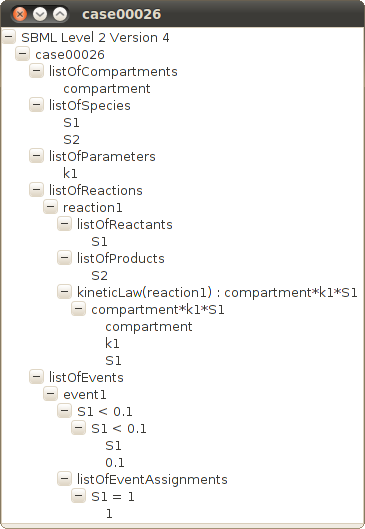
\includegraphics[width=.35\textwidth]{posters/2010_ICSB_and_COMBINE/JSBMLvisualizerTransparent}
\caption[Tree representation of an SBML file]{A tree representation of the
content of SBML test model \texttt{case00026}. In JSBML, the hierarchically
structured \texttt{SBMLDocument} can be traversed recursively because all
instances of \texttt{SBase} implement the interface \texttt{TreeNode}.}
\label{fig:Visualization}
\end{SCfigure}

Listing~\vref{lst:Visualization} demonstrates in a simple code example how to parse an SBML file\index{SBML!XML file} (submitted as first argument) and to immediately display its content on a \texttt{JFrame}\index{graphical user interface!\texttt{JFrame}}.
Fig.~\vref{fig:Visualization} shows an example output when applying the program to an SBML test model\index{SBML!test cases}.
Line 19 in Listing \ref{lst:Visualization} shows how to read an \texttt{SBMLDocument} from a file, using the \texttt{SBMLReader}. Afterwards, the \texttt{SBMLvisualizer} constructor is called, which first creates a new \texttt{JFrame} with the model's id as title (line 10). Since JSBML's \texttt{SBase} object, and all derived elements, implement the \texttt{TreeNode} interface, it is possible to create a \texttt{JTree} simply on the \texttt{SBMLDocument}, which is done in line 11.

\subsection{Creating and writing an \texttt{SBMLDocument}}
\lstinputlisting[language=Java,float,caption={Creating a new \texttt{SBMLDocument} and writing its content to disk},label=lst:Creation]{JSBMLexample.java}

Listing~\vref{lst:Creation} shows a more complex example. A new \texttt{SBMLDocument} is created from scratch. It mainly consists of one \texttt{Compartment}, one \texttt{Model}, two \texttt{Species}, and a \texttt{Reaction} in which both \texttt{Species} are involved. This \texttt{SBMLDocument} is written to the disk, using the \texttt{SBMLWriter}.

\subsection{Further examples}
Listing~\vref{lst:LibSBMLio} shows how to convert libSBML data structures into JSBML data objects. Listing~\vref{lst:PluginAction} demonstrates the implementation of CellDesigner's abstract class \texttt{PluginAction} and Listing ~\vref{lst:Plugin} gives a complete example for writing CellDesigner plugins with JSBML.


\chapter{Main differences between JSBML and libSBML}

Until today, libSBML was the main library for developing Java applications that use SBML. Thus, many Java developers are used to the methods and commands, libSBML provides. The JSBML team made some effort to allow those developers a fast and easy switch to libSBML. For example, a libSBML compatibility module has developed, that implements existing libSBML methods and simply redirects the parameters to the corresponding JSBML methods. But it is important that developers, coming from libSBML, know the main differences between the two libraries. The following sections give a brief description of those main differences.

\section{Introduction}

The intention of implementing a pure Java\texttrademark{}
Application Programming Interface (API) for working with SBML files was not to
re-implement the existing Java API of libSBML\index{application programming interface!libSBML} \citep{Bornstein2008}.
From the very beginning, JSBML\index{application programming interface!JSBML}
has been designed based on the SBML specifications \citep{Hucka2003, Hucka2008,
Hucka2010a} but with respect to naming conventions of methods and variables from
libSBML. Similarly to the SBML specifications\index{SBML!specification},the
libSBML library has grown
historically. The implementation of JSBML permitted to entirely
re-design the type hierarchy of the SBML elements and the way to
implement what is specified in the SBML specifications. However, it is important
to keep in mind that SBML is a
language that defines how to store and to exchange models of biological
processes between\index{model!storage and exchange} different software tools. It
does not specify how to represent its elements in memory. Furthermore, during
the evolution of SBML some elements or properties of elements have become
obsolete\index{deprecation}.
It is therefore up to an implementing library to
decide how to deal with those constructs. To facilitate switching from libSBML
to JSBML and the other way around, JSBML has been designed to behave similarly
to libSBML but, due to the different background of both libraries and the fact
that libSBML is based on \texttt{C}\index{C@\texttt{C}}
and \texttt{C++}\index{C++@\texttt{C++}} code, some differences are
unavoidable. In cases of doubt JSBML tries to mirror the SBML specifications
rather than libSBML. Finally, JSBML has also been developed as a library that
does not ``only" provide reading, manipulating, and writing abilities for SBML
files. It is intended to be directly used as a flexible internal data structure
for numerical computation, visualization and much more. With the help of its
modules JSBML can also be used as a communication layer between applications,
such as CellDesigner \citep{Funahashi2003}. The
following sections will not only give a detailled overview about the most
important differences between JSBML and libSBML, but also provide some programming
examples and hints about how to use and work with JSBML.


\section{An extended type hierarchy}

Whenever multiple elements defined in at least one of the SBML\index{SBML}
specifications\index{SBML!specification} share some
attributes, JSBML\index{JSBML!type hierarchy} provides a common superclass or at
least a common interface that gathers methods for the manipulation of the shared
properties. In this way, the type hierarchy of JSBML\index{application programming interface!JSBML} has become quite complex (see
Figs.~\vrefrange{fig:TypeHierarchy}{fig:MathContainerHierarchy}).
\begin{sidewaysfigure}[htbp]
\centering
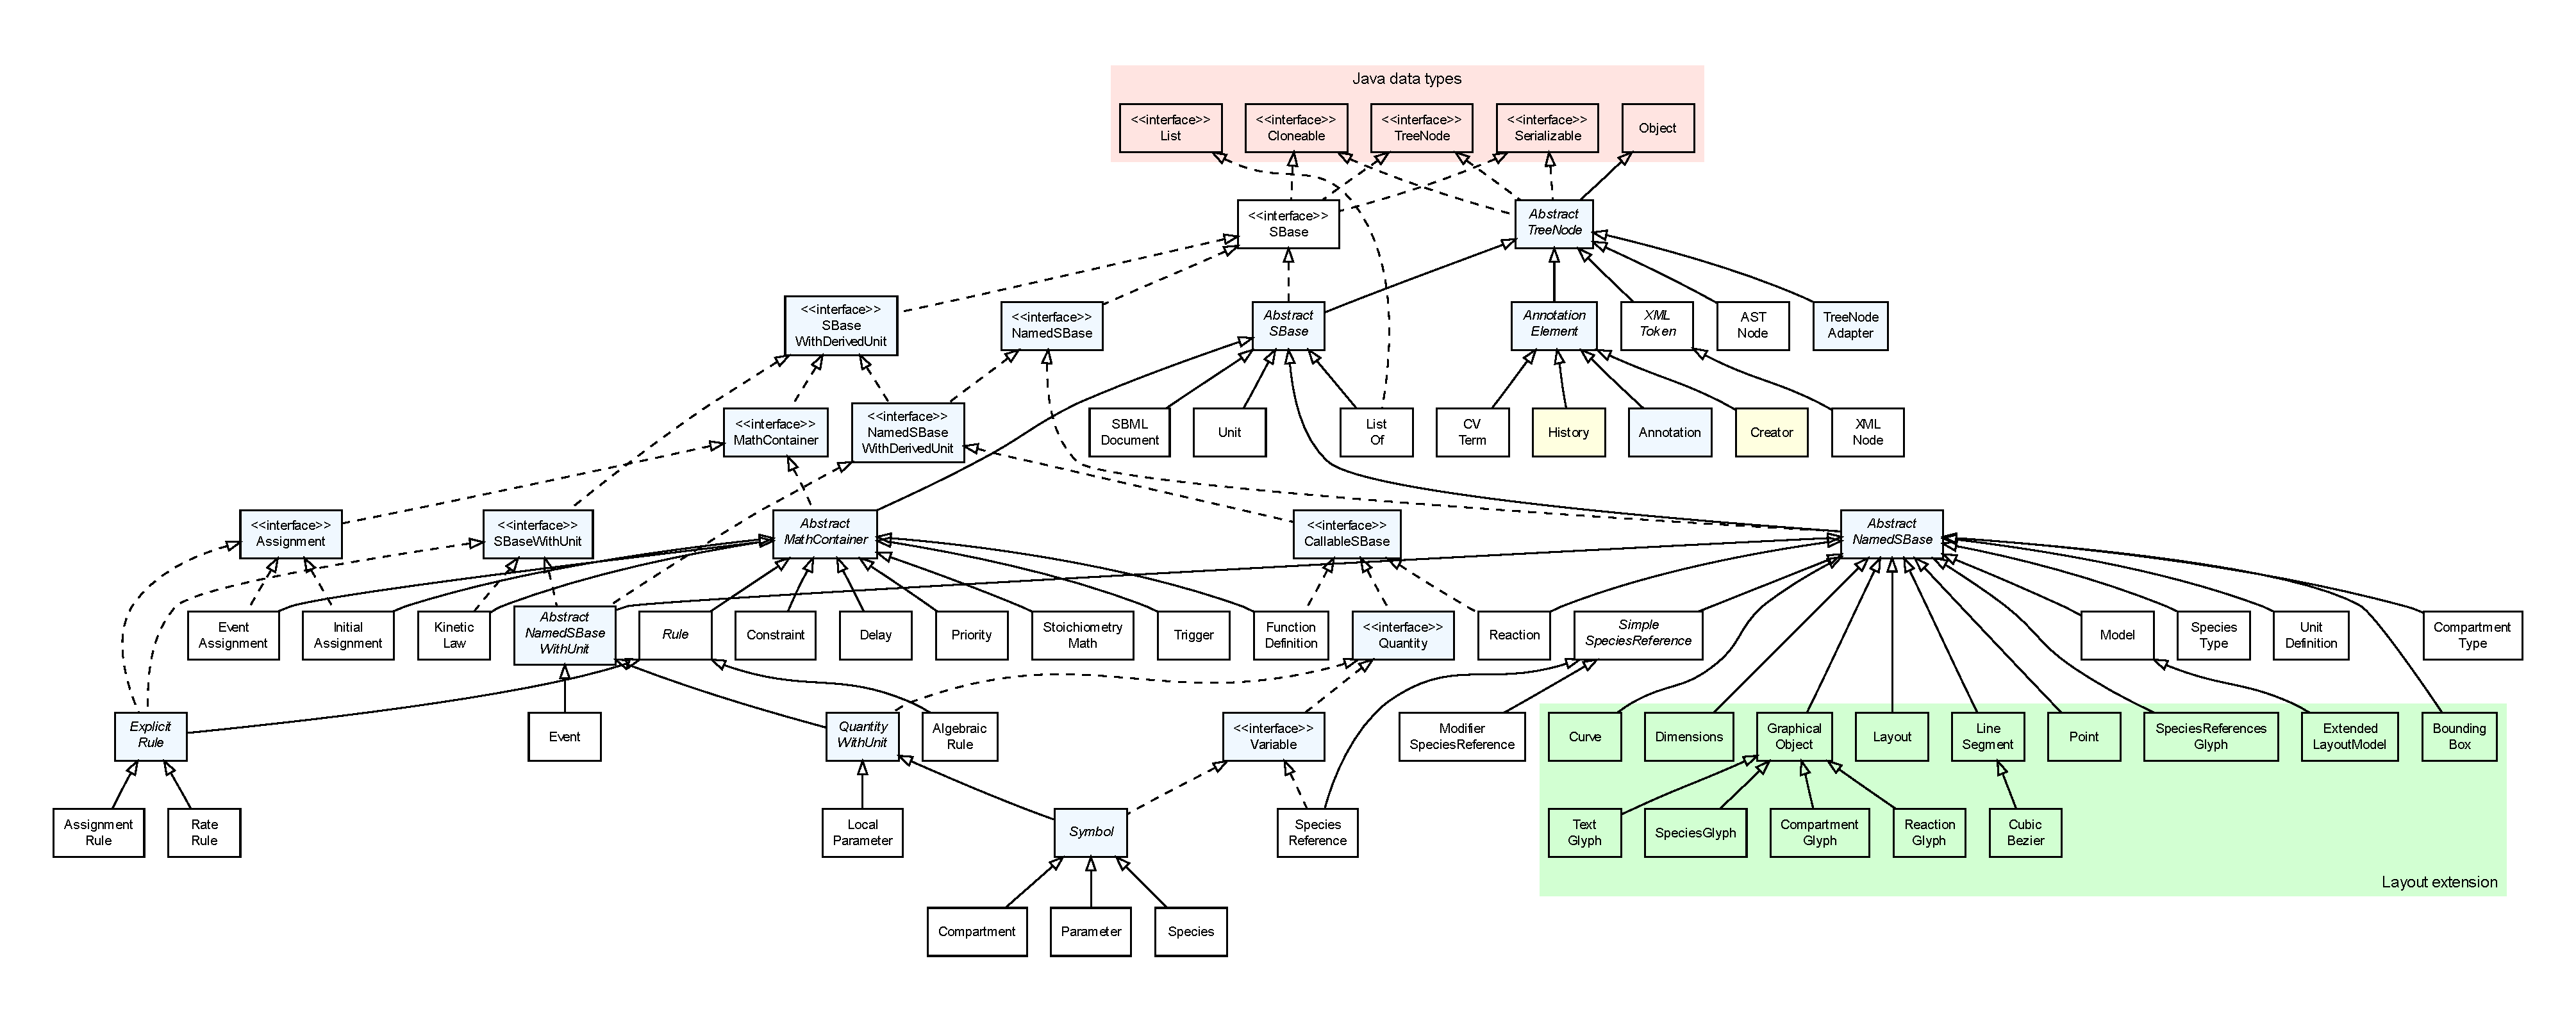
\includegraphics[width=\textwidth]{img/FullTypeHierarchy.pdf}
\caption[The type hierarchy of the main SBML
constructs in JSBML]{The type hierarchy of the main SBML
constructs in JSBML.

% N�chster satz auch schon oben verwendet.
With letting \texttt{SBase} implement the Java interfaces
\texttt{Cloneable}, \texttt{Serializable}, and \texttt{TreeNode}, all derived
elements also implement these types. Elements colored in blue have been
introduced as additional, in most cases abstract, data types in JSBML but do not
have a corresponding element in libSBML. The yellow types \texttt{Creator} and
\texttt{History} correspond to \texttt{ModelCreator} and \texttt{ModelHistory}
in libSBML.}
\label{fig:TypeHierarchy}
\end{sidewaysfigure}
\begin{figure}[htb]
 \centering
 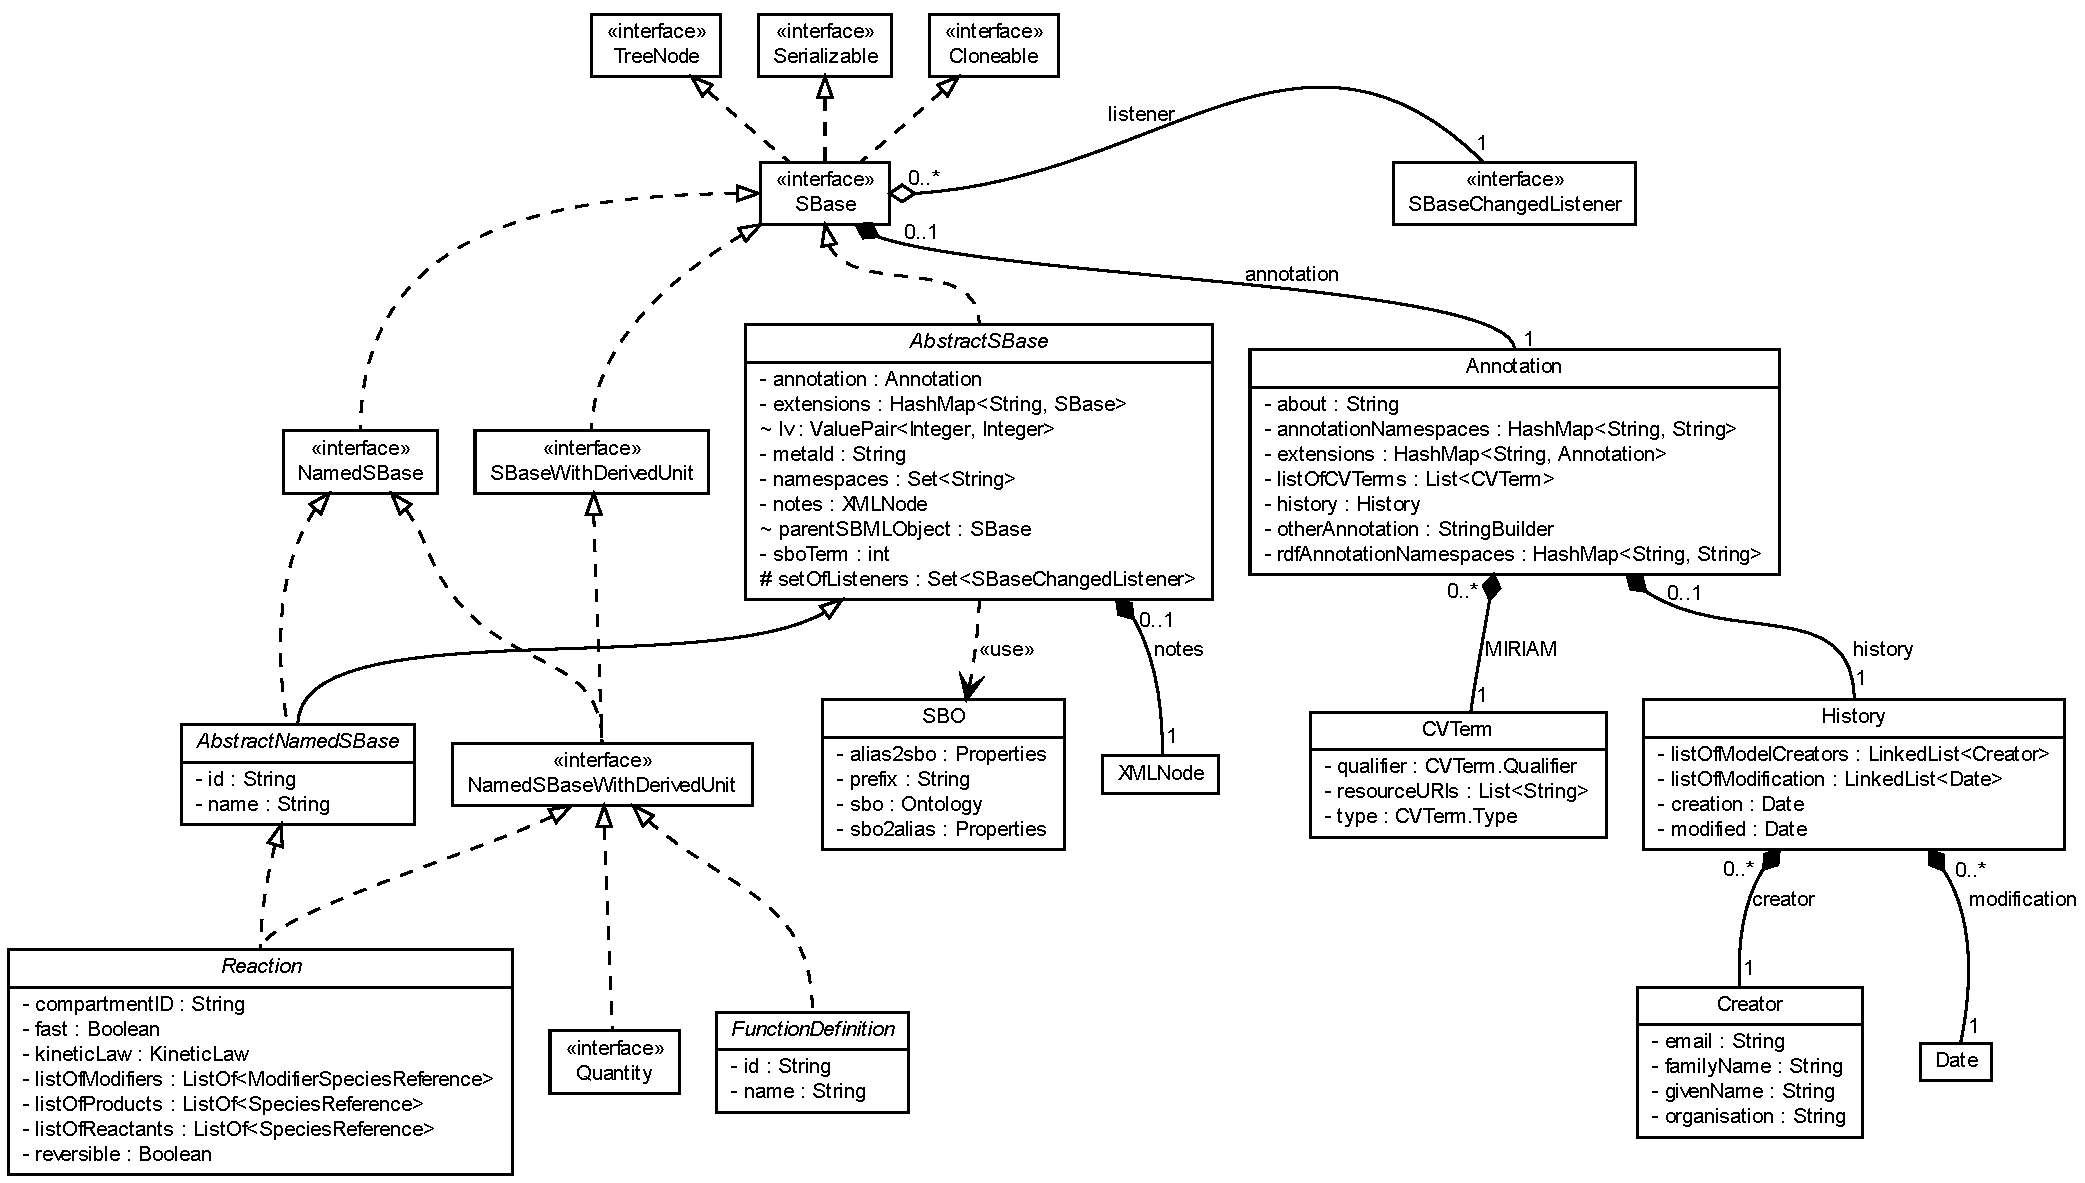
\includegraphics[width=\textwidth]{img/SBase}
 % SBase.pdf: 1001x568 pixel, 72dpi, 35.31x20.04 cm, bb=0 0 1001 568
 \caption[The interface \texttt{SBase}]{The interface \texttt{SBase}, adapted
from \citep{Draeger2011}. This figure displays the most important top-level data
structures of JSBML with main focus on the differences to libSBML. All other
data types that represent SBML constructs in JSBML extend either one of the two
abstract classes \texttt{AbstractSBase} or \texttt{AbstractNamedSBase}. The
class \texttt{SBO} parses the ontology file provided on the SBO web
site (\url{http://www.ebi.ac.uk/sbo/main/}) in OBO format (Open
Biomedical Ontologies) using a parser provided by the BioJava project
\citep{Holland2008}. For the sake of a clear arrangement, this figure omits
methods, fields and other properties.}
 \label{fig:SBase}
\end{figure}
\begin{figure}[p]
 \centering
 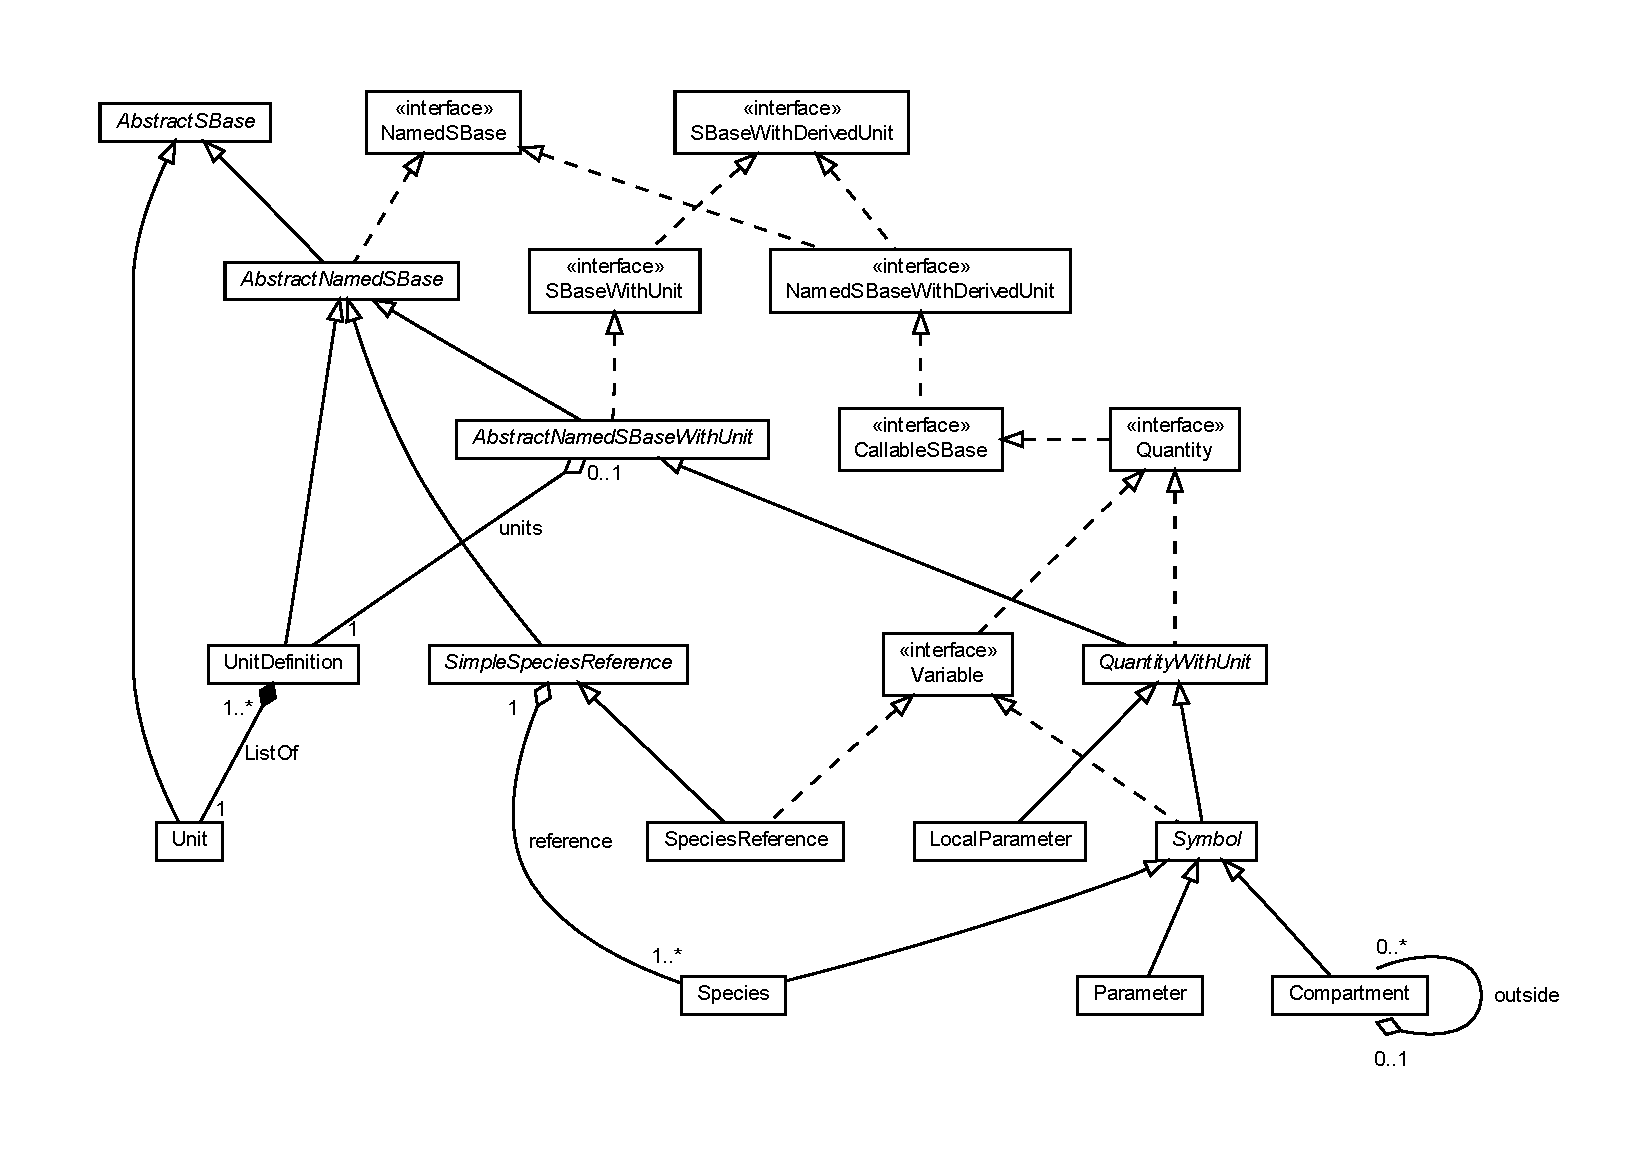
\includegraphics[width=\textwidth]{img/Symbol}
 % Symbol.pdf: 596x587 pixel, 72dpi, 21.03x20.71 cm, bb=0 0 596 587
 \caption[The interface \texttt{Variable}]{The interface \texttt{Variable}, adapted from \citep{Draeger2011}. JSBML refers to those components of a model that may change their value during a simulation as \texttt{Variable}s. The class \texttt{Symbol} serves as the abstract superclass for variables that can also be equipped with a unit. Instances of \texttt{Parameter} do not contain any additional field. In \texttt{Species}, a Boolean switch decides whether its value is to be interpreted as an initial amount or as an initial concentration. In contrast to \texttt{Variable}s, \texttt{LocalParameter}s represent constant unit-value pairs that can only be accessed within their declaring \texttt{KineticLaw}.}
 \label{fig:Variable}
\end{figure}
\begin{figure}[t!]
 \centering
 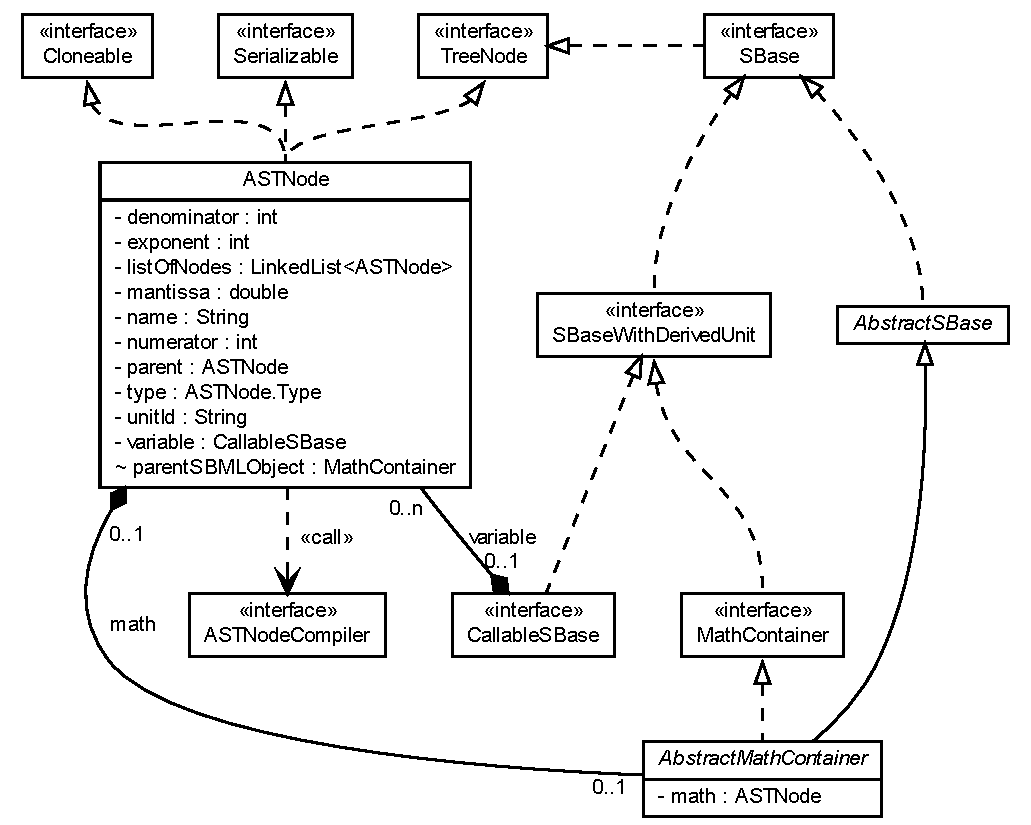
\includegraphics[width=.8\textwidth]{img/MathContainerClass}
 % MathContainerClass.pdf: 557x396 pixel, 72dpi, 19.65x13.97 cm, bb=0 0 557 396
 \caption[Abstract syntax trees]{Abstract syntax trees, adapted from
 \citep{Draeger2011}. The class \texttt{AbstractMathContainer} serves as the
 superclass for several model components in JSBML. It provides methods to
 manipulate and access an instance  of \texttt{ASTNode}, which can be converted
 to or read from \texttt{C}-like formula \texttt{String}s. Internally,
 \texttt{AbstractMathContainer}s only deal with instances of \texttt{ASTNode}.
 It should be noted that these abstract syntax trees do not implement the
 \texttt{SBase} interface, but implement the Java interfaces
 \texttt{Cloneable}, \texttt{Serializable}, and \texttt{TreeNode}. In this
 figure, the inheritance relationship between
 \texttt{SBase} and \texttt{Cloneable} as well as between \texttt{SBase} and
 \texttt{Serializable} has been omitted for the sake of simplicity.}
 \label{fig:MathContainer}
\end{figure}
\begin{figure}[htb]
 \centering
 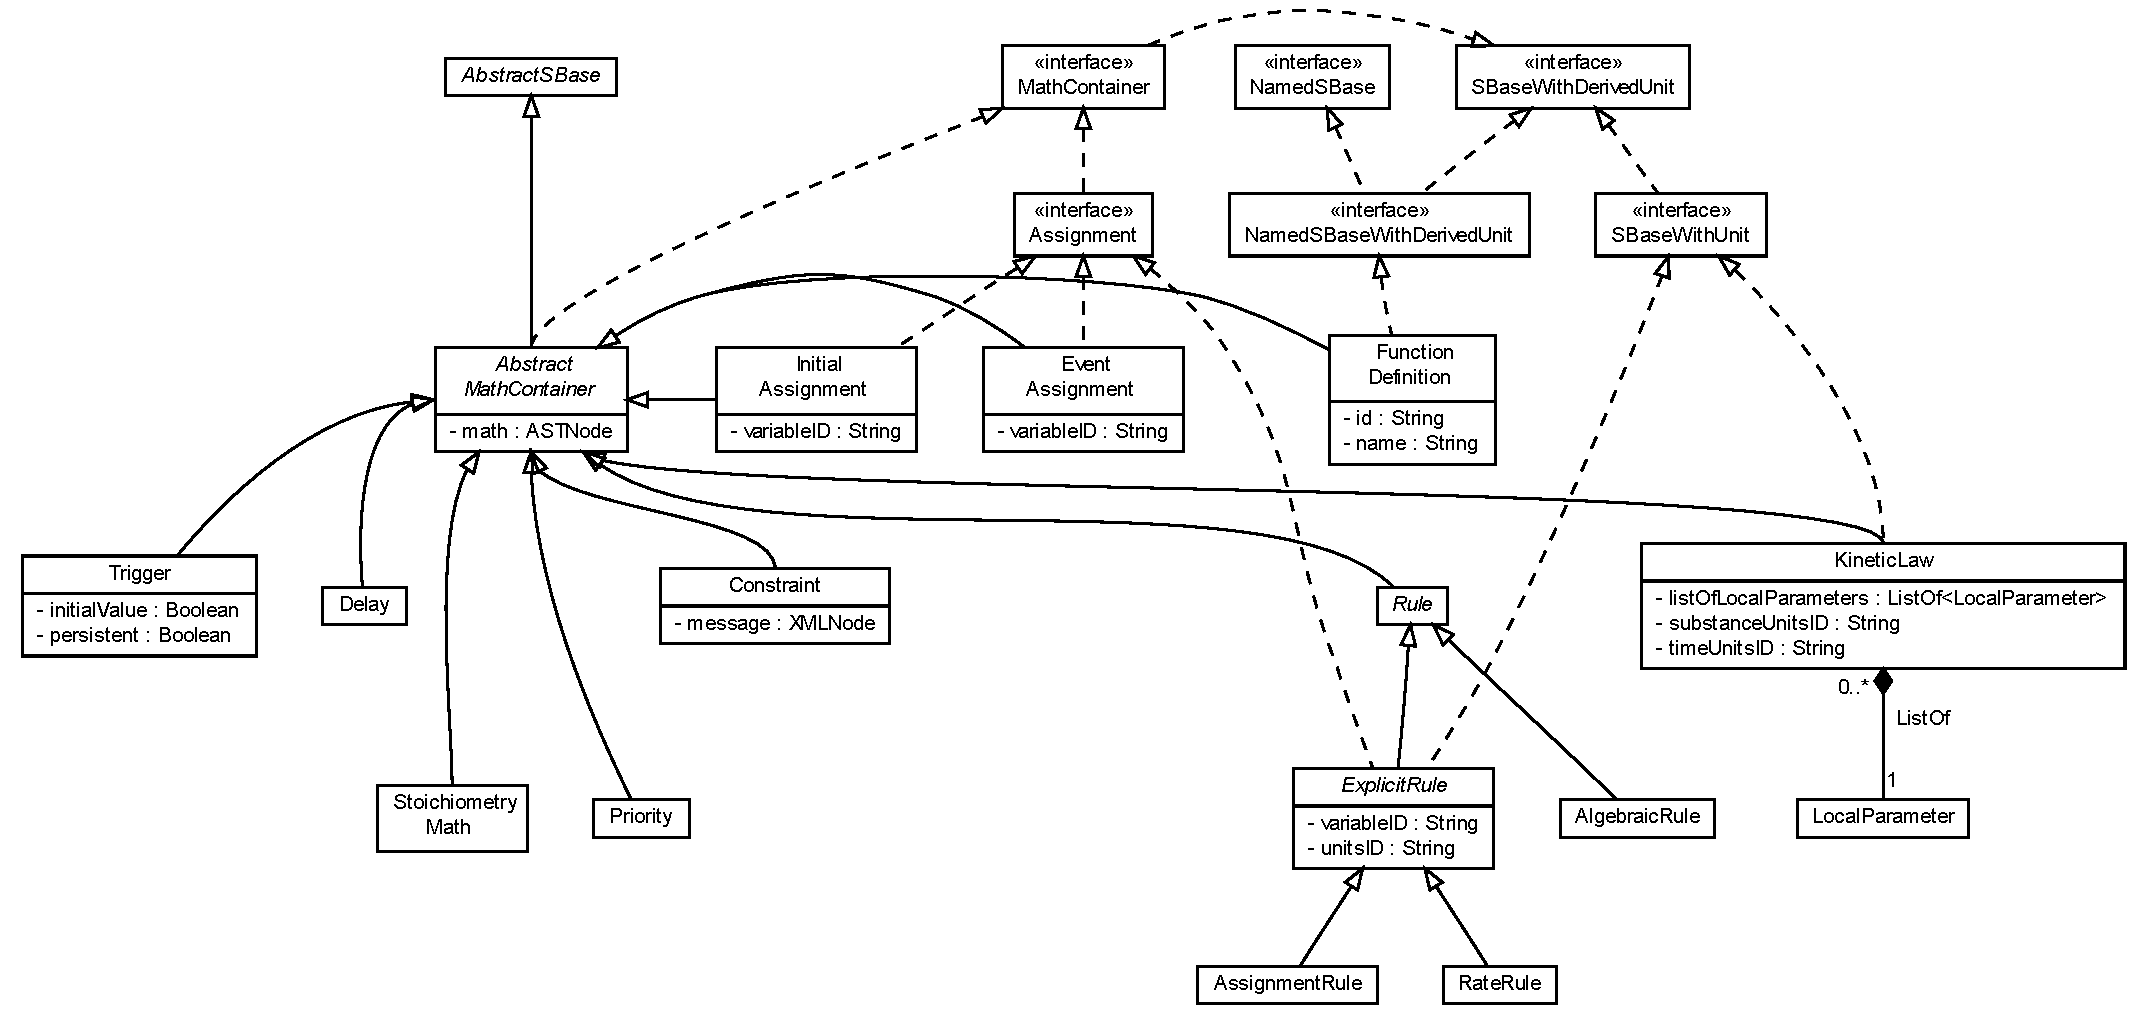
\includegraphics[width=\textwidth]{img/MathContainer}
 % MathContainerClass.pdf: 557x396 pixel, 72dpi, 19.65x13.97 cm, bb=0 0 557 396
 \caption[\texttt{MathContainer}]{\texttt{MathContainer}, adapted from
 \citep{Draeger2011}. Instances of the interface \texttt{MathContainer},
 particularly its directly derived class \texttt{AbstractMathContainer},
 constitute the superclass for all elements that store and manipulate
 mathematical formulas in JSBML, which is done in form of \texttt{ASTNode}
 objects. These can be evaluated using an implementation of
 \texttt{ASTNodeCompiler}. Note that some classes that extend
 \texttt{AbstractMathContainer} do not contain any own fields or methods:
 \texttt{Delay}, \texttt{Priority}, \texttt{StoichiometryMath}, or
 \texttt{AlgebraicRule}.}
 \label{fig:MathContainerHierarchy}
\end{figure}
Just as in libSBML\index{application programming interface!libSBML}, all elements extend the abstract type \texttt{SBase},
\index{SBase@\texttt{SBase}} but in JSBML, \texttt{SBase}
has become an interface. This allows more complex relations
between derived data types. In contrast to libSBML, \texttt{SBase} in JSBML
extends three other interfaces: \texttt{Cloneable}, \texttt{Serializable},
\index{Serializable@\texttt{Serializable}} and \texttt{TreeNode}. As all
elements defined in JSBML\index{cloning} override the \texttt{clone()}
method from the class \texttt{java.lang.Object},\index{Object@\texttt{Object}}
all JSBML elements can be deeply copied and are therefore \emph{cloneable}. By
extending the interface
\texttt{Serializable}\index{Serializable@\texttt{Serializable}}, it is possible
to store JSBML\index{application programming interface!JSBML} elements in
binary form without explicitly writing them to an SBML file\index{SBML!XML file}.
In this way, programs can easily load and save their in-memory objects or send complex data structures
through a network connection without the need of additional file encoding and
subsequent parsing. The third interface, \texttt{TreeNode} is actually defined
in Java's \texttt{swing}\index{graphical user interface!\texttt{swing}} package.
\texttt{TreeNode} is a type that is independent of any graphical information. It basically defines recursive methods on hierarchically structured data types, such as iteration
over all of its successors. In this way, all instances of
JSBML's\index{SBase@\texttt{SBase}} \texttt{SBase} interface can be directly passed to
the \texttt{swing}\index{graphical user interface!\texttt{swing}} class
\texttt{JTree}\index{graphical user interface!\texttt{JTree}} and hence be
easily visualized. Listing~\vref{lst:Visualization} demonstrates in a simple code example how to
parse an SBML file\index{SBML!XML file} and to immediately display its content
on a \texttt{JFrame}\index{graphical user interface!\texttt{JFrame}}.

The \texttt{ASTNode} class in JSBML\index{ASTNode@\texttt{ASTNode}} also implements all these three interfaces and
can hence be cloned, serialized, and visualized in the same way.


\subsection{\texttt{SBase}s with names, values and units}

The SBML\index{SBML} specifications define the data type
\texttt{SBase}\index{SBase@\texttt{SBase}}\index{SBML!specification} as the
supertype for all other SBML elements. In JSBML, \texttt{SBase} has become an
interface and most elements therefore extend its abstract implementation
\texttt{AbstractSBase}\index{SBase@\texttt{SBase}!\texttt{AbstractSBase}}.

Some types derived from \texttt{SBase} contain a unique identifier, an
\texttt{id}. JSBML gathers all these elements under the common interface
\texttt{NamedSBase}. The class \texttt{AbstractNamedSBase}, which extends
\texttt{AbstractSBase}, implements this interface.
\index{SBase@\texttt{SBase}!\texttt{NamedSBase}}
\index{SBase@\texttt{SBase}!\texttt{AbstractNamedSBase}}

Many SBML elements represent some quantitative value, which is associated with a
unit. However, the value does not necessarily have to be defined explicitly. In
many cases, it needs to be computed from a formula contained in the instance of
\texttt{SBase} in form of an abstract syntax tree, i.e., \texttt{ASTNode}.
\index{ASTNode@\texttt{ASTNode}}
Therefore, also the associated unit may not be set explicitly but can be derived
when evaluating the formula. In JSBML, the interface
\texttt{SBaseWithDerivedUnit}
\index{SBase@\texttt{SBase}!\texttt{SBaseWithDerivedUnit}}
unifies all those elements
that either explicitly or implicitly contain some unit. If these elements can
also be addressed using an identifier, they also implement the interface
\texttt{NamedSBaseWithDerivedUnit}.
\index{SBase@\texttt{SBase}!\texttt{NamedSBaseWithDerivedUnit}}
Within formulas, i.e., \texttt{ASTNode}s,
references can only be made to instances of \texttt{CallableSBase},
\index{JSBML!CallableSBase@\texttt{CallableSBase}}
which is a
special case of \texttt{NamedSBaseWithDerivedUnit}.
Fig.~\vref{fig:Variable} shows this part of JSBML's type hierarchy in more
detail.

As a special case, these elements may explicitly declare a unit. The interface
\texttt{SBaseWithUnit}
\index{SBase@\texttt{SBase}!\texttt{SBaseWithUnit}}
serves as the supertype for all those elements that may
be explicitly equipped with a unit. The convenient class
\texttt{AbstractNamedSBaseWithUnit}
\index{SBase@\texttt{SBase}!\texttt{AbstractNamedSBaseWithUnit}}
\index{SBase@\texttt{SBase}!\texttt{AbstractNamedSBase}}
extends \texttt{AbstractNamedSBase} and
implements both interfaces \texttt{SBaseWithUnit} and
\index{SBase@\texttt{SBase}!\texttt{SBaseWithUnit}}
\texttt{NamedSBaseWithDerivedUnit}.
\index{SBase@\texttt{SBase}!\texttt{NamedSBaseWithDerivedUnit}}
All elements derived from this abstract
class may therefore declare a unit and can be addressed using a unique
identifier.

Furthermore, the interface \texttt{Quantity}
\index{JSBML!quantity@\texttt{Quantity}}
describes an element that is associated with a value and at least a derived
unit. In addition, a \texttt{Quantity} can be addressed
using its unique identifier. JSBML uses the term \texttt{QuantityWithUnit} for
a \texttt{Quantity} that explicitly declares its unit. In contrast to
\texttt{Quantity}, the data type \texttt{QuantityWithUnit}
\index{JSBML!quantityWithUnit@\texttt{QuantityWithUnit}}
is not an interface, but an abstract class.

If a \texttt{Quantity} provides a Boolean
\index{Boolean}
switch to decide whether it describes a constant,
\index{constant}
JSBML represents such a type in the interface \texttt{Variable}.
\index{JSBML!variable@\texttt{Variable}}
Finally, JSBML refers to \texttt{Variable}s with a defined unit as a
\texttt{Symbol}
\index{JSBML!symbol@\texttt{Symbol}}
and provides a corresponding abstract class. In this way, the
SBML elements \texttt{Compartment}, \texttt{Parameter}, and \texttt{Species}
\index{compartment!\texttt{Compartment}}
\index{parameter!\texttt{Parameter}}
\index{species!\texttt{Species}}
are special cases of \texttt{Symbol} in JSBML. The specification of SBML Level~3
\index{SBML!Level~3}
introduces another type of \texttt{Variable}, which does not explicitly declare
its unit: \texttt{SpeciesReference}. On the other hand, a
\texttt{LocalParameter}
\index{parameter!\texttt{LocalParameter}}
is a \texttt{QuantityWithUnit},
\index{JSBML!quantityWithUnit@\texttt{QuantityWithUnit}}
but not a \texttt{Variable}, because it is always constant.
\index{constant}


\subsection{The \texttt{MathContainer} interface}

This interface gathers all those elements that may contain mathematical
expressions encoded in abstract syntax trees (instances of
\texttt{ASTNode}\index{ASTNode@\texttt{ASTNode}}).
The abstract class \texttt{AbstractMathContainer}
\index{JSBML!MathContainer@\texttt{MathContainer}}
serves as actual superclass
for most of the derived types.
Figs.~\vrefrange{fig:MathContainer}{fig:MathContainerHierarchy} give a better
overview of how this data structure is intended to function.


\subsection{The \texttt{Assignment} interface}

JSBML
\index{JSBML!assignment@\texttt{Assignment}}
unifies all those elements that may
change the value of some \emph{variable} in SBML\index{SBML} under the interface
\texttt{Assignment}. This interface uses the term \emph{variable}
for the element whose value is to be changed
depending on some mathematical expression that is also present in the
\texttt{Assignment} (because \texttt{Assignment} extends the interface
\texttt{MathContainer}).
\index{JSBML!MathContainer@\texttt{MathContainer}}
Therefore,
an \texttt{Assignment} contains methods such as
\texttt{set}-/\texttt{getVariable(Variable v)} and also \texttt{isSetVariable()}
as well as \texttt{unsetVariable()}. In addition to that, JSBML also provides
the method \texttt{set}-/\texttt{getSymbol(String symbol)} in the
\texttt{InitialAssignment}
\index{InitialAssignment@\texttt{InitialAssignment}}
class to make sure that switching from libSBML
to JSBML is quite smoothly.
However, the preferred way in JSBML
\index{JSBML!variable@\texttt{Variable}}
is to apply the methods \texttt{setVariable} either with \texttt{String}
\index{string@\texttt{String}!identifier}
or \texttt{Variable} instances as arguments.
Fig.~\vref{fig:MathContainerHierarchy} displays the type hierarchy of the
\texttt{Assignment} interface in more detail.



\section{Differences in the abstract programming interface}

JSBML strives to attain an almost complete compatibility to libSBML. However,
the differences in the programming languages \texttt{C++}
\index{C++@\texttt{C++}}
and Java\texttrademark{} lead to the necessity of introducing some differences.
In some cases, a direct ``translation" from \texttt{C++} and \texttt{C} code to
\index{C@\texttt{C}}
Java would not be very elegant. JSBML wants to provide a Java
API\index{application programming interface!Java}, whose classes and methods are
structured and named and behave like classes and methods in other Java
libraries. In this section, we will discuss the most important differences in
the APIs of JSBML\index{application programming interface!JSBML} and
libSBML\index{application programming interface!libSBML}.


\subsection{Abstract syntax trees}

Both libraries define a class \texttt{ASTNode}\index{ASTNode@\texttt{ASTNode}} for in-memory manipulation and
evaluation of abstract syntax trees that represent mathematical formulas and
equations. These can either be parsed from a representation in \texttt{C}
language-like \texttt{String}s\index{string@\texttt{String}!formula}, or from a MathML\index{MathML} representation. The JSBML\index{ASTNode@\texttt{ASTNode}}
\texttt{ASTNode} provides various methods to transform these trees to other
formats, for instance, \LaTeX{}
\index{LaTeX@\LaTeX} \texttt{String}s. In JSBML, several static
methods allow easy creation of new syntax trees, for instance, the following
code
\begin{lstlisting}[language=Java,numbers=none]
ASTNode myNode = ASTNode.plus(myLeftAstNode, myRightASTNode);
\end{lstlisting}
creates a new instance of \texttt{ASTNode} which represents the sum of the two
other \texttt{ASTNode}s. In this way, even complex trees can be easily
manipulated.

\textcolor{red}{There is more change than this, we have methods that take/return
CallableSBase}

\subsection{The \texttt{ASTNodeCompiler} class}

This interface allows users to create customized interpreters for the
content of mathematical equations encoded in abstract syntax trees. It
is directly and recursively called from the \texttt{ASTNode} class and returns
an \texttt{ASTNodeValue}
\index{ASTNode@\texttt{ASTNode}!\texttt{ASTNodeValue}}
\index{ASTNode@\texttt{ASTNode}!\texttt{ASTNodeCompiler}} object,
which wraps the possible evaluation results of the interpretation.
JSBML\index{ASTNode@\texttt{ASTNode}} already provides several implementations of this
interface, for instance, \texttt{ASTNode} objects can be directly translated to
\texttt{C} language-like \texttt{String}s\index{string@\texttt{String}!formula},
\LaTeX,\index{LaTeX@\LaTeX} or MathML\index{MathML} for further processing.
Furthermore, the class \texttt{UnitsCompiler},
\index{unit!UnitsCompiler@\texttt{\texttt{UnitsCompiler}}}
which JSBML uses to derive the unit of an abstract syntax tree, also implements
this interface.

\subsection{Cloning when adding child nodes}

When adding elements such as a \texttt{Species}\index{species!\texttt{Species}} to a \texttt{Model}\index{model!\texttt{Model}}, libSBML\index{cloning} will clone the object and add the clone to the \texttt{Model}. In contrast, JSBML\index{cloning} does
not automatically perform cloning. The advantage is that modifications on the
object belonging to the original pointer will also propagate to the element
added to the \texttt{Model}. Furthermore, this is more efficient with respect to
the run time and also more intuitive for java programmers. If cloning is
necessary, users should call the \texttt{clone()} method manually. Since all instances of \texttt{SBase}\index{SBase@\texttt{SBase}} and also
\texttt{Annotation}\index{annotation}, \texttt{ASTNode}\index{ASTNode@\texttt{ASTNode}}, \texttt{CVTerm}\index{annotation!\texttt{CVTerm}}, and \texttt{History}\index{annotation!\texttt{History}} implement
the interface \texttt{Cloneable}\index{cloning} (see Fig.~\vref{fig:TypeHierarchy}), all these
elements can be naturally cloned. However, when cloning an object in
JSBML\index{cloning}, such as an \texttt{AbstractNamedSBase},
\index{SBase@\texttt{SBase}!\texttt{AbstractNamedSBase}}
all children of this element will recursively be cloned before adding them to
the new element. This is necessary, because the data structures specified in
SBML
\index{SBML!hierarchical structure}
define a tree, in which each element has exactly one parental node.

\subsection{Compartments}

In SBML Level 3\index{SBML!Level~3} \citep{Hucka2010a}, the domain of the
\texttt{spatialDimensions} attribute in \texttt{Compartment}s
was changed from $\lbrace 0, 1, 2, 3\rbrace$, which can be represented with a
\texttt{short} value in Java to a value in $\mathbb{R}$, i.e., a \texttt{double}
value. For this reason, the method \texttt{getSpatialDimensions()} in JSBML
always returns a \texttt{double} value. For consistency with libSBML, the
\texttt{Compartment} class in JSBML also provides the redundant method
\texttt{getSpatialDimensionsAsDouble()} that returns the identical value, but
that is marked as a deprected method.
\index{compartment}
\index{compartment!\texttt{getSpatialDimensions()}}
\index{compartment!\texttt{getSpatialDimensionsAsDouble()}}


\subsection{Deprecation}

The intention of JSBML\index{JSBML!deprecation} is to provide a Java library
that support the latest specifications of SBML\index{SBML}.
\index{SBML!specification}
\index{deprecation}
But we also want to support earlier specifications. So JSBML provides methods
and classes to cover those as well, but these are often marked
as being deprecated to avoid creating models that refer to these
elements.

\subsection{Exceptions}

In case of an error, JSBML\index{exception} throws often an exception while
libSBML\index{exception!error codes} methods return some error codes instead.
This behavior helps programmers and users to avoid creating invalid SBML data structures already
when dealing with these in memory. Furthermore, exception handling is very well
implemented in Java and it is therefore a better programming style in this
language. Methods can already declare that these may potentially throw
exceptions. In this way, programmers can be aware of potential sources of
problems already at the time of writing the source code.
Examples are the \texttt{ParseException}
\index{exception!\texttt{ParseException}} that
may be thrown if a given formula cannot be parsed properly into an
\texttt{ASTNode}\index{ASTNode@\texttt{ASTNode}} data structure, or \texttt{InvalidArgumentException}s
\index{exception!\texttt{InvalidArgumentException}} if inappropriate values are passed to methods. For instance,
\begin{itemize}
 \item An object representing a constant\index{constant} such as a
 \texttt{Parameter} whose \texttt{constant} attribute has been set to
\texttt{true} cannot be used as the \texttt{Variable} element in an
\texttt{Assignment}.
\index{JSBML!assignment@\texttt{Assignment}}
\index{JSBML!variable@\texttt{Variable}}
\index{parameter!\texttt{Parameter}}
\index{parameter!\texttt{constant}}
 \item An instance of \texttt{Priority}\index{event!\texttt{Priority}} can only be assigned to an \texttt{Event}s\index{event!\texttt{Event}} if its \texttt{level}\index{SBML!Level~3} attribute has at least been set to three.
 \item Another example is the \texttt{InvalidArgumentException} that
is thrown when trying to set an invalid identifier \texttt{String} for an instance of \texttt{AbstractNamedSBase}.
\index{SBase@\texttt{SBase}!\texttt{AbstractNamedSBase}}
\end{itemize}
Hence, you have to be aware of potential
exceptions and errors when using JSBML\index{exception}, on the other hand this will
prevent you from doing obvious mistakes. One potential problem of detecting
errors quickly and throwing exceptions is that it might prevent JSBML to be able
to read properly invalid SBML models.


\subsection{Model history}

In earlier versions of SBML\index{SBML}, only the model itself could be
associated with a history, i.e., a description about the person(s) who build
this model, including names, e-mail addresses, modification and creation dates.
Nowadays, it has become possible to annotate each individual construct of an
SBML model with such a history. This is reflected by naming the corresponding
object \texttt{History}\index{annotation!\texttt{History}}
in JSBML\index{annotation!\texttt{ModelHistory}}, whereas it is still called
\texttt{ModelHistory} in libSBML\index{annotation!\texttt{ModelHistory}}. Hence,
all instances of \texttt{SBase}\index{SBase@\texttt{SBase}} in JSBML
\index{annotation!\texttt{ModelHistory}} contain methods to access and
manipulate its \texttt{History}. Furthermore, you will not find the classes
\texttt{ModelCreator} and \texttt{ModelCreatorList} because
JSBML\index{annotation!\texttt{ModelCreator}}
gathers its \texttt{Creator} objects
in a generic \texttt{List<Creator>} in the
\texttt{History}\index{annotation!\texttt{History}}.


\subsection{Replacement of the interface \texttt{libSBMConstants} by Java \texttt{enum}s}

You won't find a corresponding implementation of the interface
\texttt{libSBMConstants} in JSBML. The reason is that the JSBML team decided to
encode constants \index{constant!\texttt{enum}}
using the Java construct \texttt{enum}. For instance, all the fields starting
with the prefix \texttt{AST\_TYPE\_*}
\index{ASTNode@\texttt{ASTNode}!\texttt{AST\_TYPE\_*}}
have a corresponding field in the \texttt{ASTNode} class itself. There you can
find the \texttt{enum} \texttt{Type}
\index{ASTNode@\texttt{ASTNode}!\texttt{ASTNode.Type}}.
Instead of typing \texttt{libSBMLConstants.AST\_TYPE\_PLUS}, you would therefore
type \texttt{ASTNode.Type.PLUS}.

The same holds true for \texttt{Unit.Kind.*} corresponding to the
\texttt{libSBMLConstants.UNIT\_KIND\_*}
\index{unit!UNIT\_KIND\_*@\texttt{UNIT\_KIND\_*}}
fields.

\subsection{The classes \texttt{libSBML} and \texttt{JSBML}}

There is no class \texttt{libSBML} because this library is called
\texttt{JSBML}.
\index{libSBML!libSBML@\texttt{libSBML}}
You can therefore only find a class \texttt{JSBML}.
\index{JSBML!JSBML@\texttt{JSBML}}
This class provides some similar methods as the \texttt{libSBML} class in
libSBML, such as \texttt{getJSBMLDottedVersion()}
\index{JSBML!version} to obtain the current
version of the JSBML library, which is 0.8.* at the time of writing this
document. However, many other methods that you might expect
to find there, if you are used to libSBML, are located in the actual classes
that are related with the function. For instance, the method to convert between
a \texttt{String}\index{string@\texttt{String}!unit}
\index{unit!String@\texttt{String}}
and a corresponding \texttt{Unit.Kind}
\index{unit!Unit.Kind@\texttt{Unit.Kind}}
can be done by using the method
\begin{lstlisting}[language=Java,numbers=none]
Unit.Kind myKind = Unit.Kind.valueOf(myString);
\end{lstlisting}
In a similar way, the \texttt{ASTNode}\index{ASTNode@\texttt{ASTNode}} class provides a method to parse
\texttt{C}-like
formula \texttt{String}s\index{string@\texttt{String}!formula} according to the specification of SBML Level 1\index{SBML!Level~1}
\citep{Hucka2003} into an abstract syntax tree\index{ASTNode@\texttt{ASTNode}}. Therefore, in contrast to the
\texttt{libSBML} class, the class \texttt{JSBML}
\index{JSBML!JSBML@\texttt{JSBML}}
contains only a few methods.


\subsection{Various types of \texttt{ListOf*} classes}

% We have the method get(String) on the ListOf and libsbml does not have it on
% the main ListOf class, only on subclasses where it is possible to do it.

In JSBML, there is not a specific
\texttt{ListOf*}\index{ListOf*@\texttt{ListOf*}} class for each type of SBase
elements. We used a generic implementation
\texttt{ListOf<?~extends SBase>} that allow us to use the same class for each of
the different {ListOf*} classes defined in libSBML while keeping a type safe
class. We defined several methods that uses the \texttt{Filter} interface to
search or filter a \texttt{ListOf} object. For example, to query an instance of
\texttt{ListOf} in JSBML for names or identifiers or both, you can apply the following filter:
\begin{lstlisting}[language=Java,numbers=none]
NamedSBase nsb = myList.firstHit(new NameFilter(identifier));
\end{lstlisting}
This will give you the first element in the list with the given identifier.
Various filters are already implemented, but you can easily add your
customized filter. To this end, you only have to implement the \texttt{Filter}
\index{ListOf*@\texttt{ListOf*}!\texttt{Filter}}
interface in \texttt{org.sbml.jsbml.util.filters}\index{ListOf*@\texttt{ListOf*}!\texttt{Filter}}. There you can also find an
\texttt{OrFilter} and an \texttt{AndFilter}, which take as arguments multiple other
filters. With the \texttt{SBOFilter} you can query for certain SBO  annotations \citep{Novere2006,Novere2006b}\index{annotation!SBO} in
your list, whereas the \texttt{CVTermFilter} helps you to identify \texttt{SBase}
\index{SBase@\texttt{SBase}}
instances with a desired MIRIAM (Minimal Information Required In the Annotation of Models) annotation\index{annotation} \citep{Novere2005}. For instances of
\texttt{ListOf<Species>} you can apply the \texttt{BoundaryConditionFilter} to look
for those species\index{species!boundary condition} that operate on the boundary of the reaction system.


\subsection{Units}

Since SBML Level 3\index{SBML!Level~3} the data type of the exponent attribute in the \texttt{Unit}
class has been changed from \texttt{int} to \texttt{double} values.
JSBML
\index{unit!Unit@\texttt{Unit}}
\index{unit!getExponent()@\texttt{getExponent()}}
\index{unit!getExponentAsDouble()@\texttt{getExponentAsDouble()}}
reflects this in the method \texttt{getExponent()} by returning \texttt{double}
values only. For a better compatibility with libSBML, whose corresponding method
still returns \texttt{int} values, JSBML also provides the method
\texttt{getExponentAsDouble()}. This method returns the value from the
\texttt{getExponent()} method and is therefore absolutely redundant.

\subsection{Unit definitions}

\subsubsection{Predefined unit definitions}

A model in JSBML
\index{unit!predefined units}
always also contains all predefined units in the model
if there are any, i.e., for models encoded with SBML versions before Level
3\index{SBML!Level~3}. These can be accessed from an instance of model by calling the method
\texttt{getPredefinedUnit(String unit)}.

MIRIAM annotations\index{annotation!MIRIAM} \citep{Novere2005} have become an integral part of SBML models
since Level 2 Version 2\index{SBML!Level~2 Version~2}. Recently, the Unit
Ontology\footnote{\url{http://www.obofoundry.org/cgi-bin/detail.cgi?id=unit}}
\index{annotation!unit ontology}
(UO) has been included in the set of supported ontology and online resources of
MIRIAM. Since all the predefined units in SBML have corresponding entries in the
UO, JSBML
\index{unit!MIRIAM annotation}
automatically equips those predefined units with the correct MIRIAM
URI in form of a controlled vocabulary term (\texttt{CVTerm}) if the
Level/Version combination of the model supports MIRIAM annotations.

Note that the \texttt{enum} \texttt{Unit.Kind}
\index{unit!Unit.Kind@\texttt{Unit.Kind}}
also provides methods to directly obtain the entry from the UO that corresponds
to a certain unit kind and also to generate MIRIAM URIs accordingly. In this
way, JSBML facilitates the annotation of user-defined units and unit definitions
with MIRIAM-compliant\index{annotation!MIRIAM} information.

\subsubsection{Access to the units of an element}

In JSBML, all SBML elements, that can be associated with some unit, implement
the interface \texttt{SBaseWithUnit}.
\index{SBase@\texttt{SBase}!\texttt{SBaseWithUnit}}
This interface provides methods to directly
access an object representing their unit. Currently, the following elements
implement this interface:
\begin{itemize}
 \item \texttt{AbstractNamedSBaseWithUnit}
 \item \texttt{ExplicitRule}\index{rule!\texttt{ExplicitRule}}
 \item \texttt{KineticLaw}
 \index{KineticLaw@\texttt{KineticLaw}}
\end{itemize}
Fig.~\vref{fig:TypeHierarchy} provides a better overview about the relationships
between all the classes explained here. Note that
\texttt{AbstractNamedSBaseWithUnit} serves as the abstract superclass for
\texttt{Event}\index{event} and \texttt{QuantityWithUnit}.
\index{JSBML!quantityWithUnit@\texttt{QuantityWithUnit}}
In the class \texttt{Event}, all methods
to deal with units are deprecated because the timeUnits attribute
was removed in SBML Level 2 Versions 2\index{SBML!Level~2}. The same holds true
for instances of
\texttt{ExplicitRule}\index{rule!\texttt{ExplicitRule}}
and \texttt{KineticLaw},\index{KineticLaw@\texttt{KineticLaw}}
which both can only be explicitly populated with units in SBML Level
1\index{SBML!Level~1} for \texttt{ExplicitRule} and before SBML in Level 2,
Versions 3\index{SBML!Level~2} for \texttt{KineticLaw}. In contrast,
\texttt{QuantityWithUnit}
\index{JSBML!quantityWithUnit@\texttt{QuantityWithUnit}}
serves as the abstract superclass for \texttt{LocalParameter}
\index{parameter!\texttt{LocalParameter}} and
\texttt{Symbol},
\index{JSBML!symbol@\texttt{Symbol}}
which is then again the super type of \texttt{Compartment}, \texttt{Species}, and (global) \texttt{Parameter}.
\index{compartment!\texttt{Compartment}}
\index{species!\texttt{Species}}
\index{parameter!\texttt{Parameter}}

With \texttt{SBaseWithUnit}
\index{SBase@\texttt{SBase}!\texttt{SBaseWithUnit}} being a subtype of
\texttt{SBaseWithDerivedUnit}
\index{SBase@\texttt{SBase}!\texttt{SBaseWithDerivedUnit}}
users can access the units of such an element in two different ways:
\begin{description}
 \item[\texttt{getUnit()}] This method returns the
 \texttt{String}\index{string@\texttt{String}!unit}
 \index{unit!String@\texttt{String}}
 of the unit kind or the unit definition in the model
 \index{model}
 that has been directly set by the user
 during the life time of the element. If nothing has been declared, an empty
 \texttt{String} will be delivered.
 \item[\texttt{getDerivedUnit()}] This method gives either the same result as
 \index{unit!derived unit}
 \texttt{getUnit()} if some unit has been declared explicitly, or it returns the
 predefined unit of the element for the given SBML Level/Version combination.
 Only if neither a user-defined nor a predefined unit is available, this method
 returns an empty \texttt{String}\index{string@\texttt{String}!empty}.
\end{description}
Both methods have corresponding methods to directly obtain an instance of
\texttt{UnitDefinition}
\index{unit!UnitDefinition@\texttt{UnitDefinition}}
for convenience.

However, care must be taken when obtaining an instance of
\texttt{UnitDefinition}
\index{unit!UnitDefinition@\texttt{UnitDefinition}}
from one of the classes implementing \texttt{SBaseWithUnit}
\index{SBase@\texttt{SBase}!\texttt{SBaseWithUnit}}
because it might happen that the model\index{model} containing this
\texttt{SBaseWithUnit}
\index{SBase@\texttt{SBase}!\texttt{SBaseWithUnit}}
does actually not contain the required instance of \texttt{UnitDefinition} and
the method returns a \texttt{UnitDefinition} that has just been created for
convenience from the information provided by the class. It might therefore be
useful to either check if the \texttt{Model}\index{model!\texttt{Model}}
contains this \texttt{UnitDefinition}
\index{unit!UnitDefinition@\texttt{UnitDefinition}}
or to add it to the \texttt{Model}\index{model!\texttt{Model}}.

In case of \texttt{KineticLaw}
\index{KineticLaw@\texttt{KineticLaw}}
it is even more difficult, because
SBML Level 1\index{SBML!Level~1} allows to separately set the substance unit and the time unit of
the element. To unify the API\index{application programming interface!JSBML}, we decided to also provide methods that allow
the user to simply pass one \texttt{UnitDefinition}
\index{unit!UnitDefinition@\texttt{UnitDefinition}}
or its identifier to
\texttt{KineticLaw}.
\index{KineticLaw@\texttt{KineticLaw}}
These methods then try to guess if a substance unit or time
unit is given. Furthermore, it is possible to pass a \texttt{UnitDefinition}
representing a variant of substance per time directly. In this case, the
\texttt{KineticLaw}
\index{KineticLaw@\texttt{KineticLaw}}
will memorize a direct link to this \texttt{UnitDefinition}
in the model\index{model} and also try to save separate links to the time unit and the
substance unit. However, this may cause a problem if the containing
\texttt{Model}\index{model!\texttt{Model}} does not contain separate \texttt{UnitDefinition}s for both
entries.

Generally, this approach provides a more general way to access and to manipulate
units of SBML elements.

\section{Additional features of JSBML}

The JSBML library also provides some features that cannot be found in libSBML.
This section briefly introduces its most important additional capabilities.

\subsection{Change listeners}

JSBML introduces the possibility to listen to change events in the life of an
SBML document. To benefit from this advantage, simply let your class implement
the interface \texttt{SBaseChangedListener}\index{event!\texttt{SBaseChangedListener}} and add it to the list of listeners in
your instance of \texttt{SBMLDocument}\index{SBML!\texttt{SBMLDocument}}. You only have to implement three methods
\begin{description}
 \item[\texttt{sbaseAdded(SBase sbase)}] This method notifies the listener that the given \texttt{SBase}\index{SBase@\texttt{SBase}}
   has just been added to the \texttt{SBMLDocument}
 \item[\texttt{sbaseRemoved(SBase sbase)}] The \texttt{SBase} instance passed to this method is no
   longer part of the \texttt{SBMLDocument} as it has just been removed.
 \item[\texttt{stateChanged(SBaseChangedEvent event)}] This method provides detailed information about some value
   change within the \texttt{SBMLDocument}. The object passed to this method is
   an \texttt{SBaseChangedEvent}\index{event!\texttt{SBaseChangedEvent}}, which provides information about the \texttt{SBase}\index{SBase@\texttt{SBase}}
   that has been changed, its property whose value has been changed (this is a
   \texttt{String}\index{string@\texttt{String}} representation of the name of the property), along with the
   previous value and the new value.
\end{description}
With the help of these methods, you can keep track of what your
\texttt{SBMLDocument}\index{SBML!\texttt{SBMLDocument}} does at any time. Furthermore, one could consider to make
use of this functionality in a graphical user interface\index{graphical user interface}, where the user should
be asked if he or she really wants to delete some element or to approve changes
before making these persistent. Another idea of using this, would be to write
log files\index{logging!log file} of the model\index{model} building process
automatically. To this end, JSBML already provides its implementation
\texttt{SimpleSBaseChangedListener},
\index{event!\texttt{SimpleSBaseChangedListener}} which notifies a logger about
each change.

Note that the class \texttt{SBaseChangedEvent}\index{event!\texttt{SBaseChangedEvent}} implements the class
\texttt{java.util.EventObject}\index{event!\texttt{EventObject}} and that the interface
\texttt{SBaseChangedListener}\index{event!\texttt{SBaseChangedListener}}\index{event!\texttt{SBaseChangedListener}} extends the interface
\texttt{java.util.EventListener}\index{event!\texttt{EventListener}}. In this way, the event and listener data
structures fit into the common Java\texttrademark{} API (Application Programming Interface)\index{application programming interface!Java} and
allow users also to make use of, e.g., \texttt{EventHandler}s\index{event!\texttt{EventHandler}} to deal with
changes in a model\index{model}. It should also be noted that \texttt{SBaseChangedListener}s
only keep track of changes in instances of \texttt{SBase} directly. This means
that changes inside of, e.g., \texttt{CVTerm}\index{annotation!\texttt{CVTerm}} or \texttt{History}\index{annotation!\texttt{History}} may not be
traced.

\subsection{Determination of the variable in \texttt{AlgebraicRule}s}

The class \texttt{OverdeterminationValidator}
\index{JSBML!OverdeterminationValidator@\texttt{OverdeterminationValidator}}
in JSBML provides methods to
determine if a model\index{model!over determination}
is over determined. This is done using the algorithm of \citet{Hopcroft1973}.
While doing that, it also determines the variable element for each
\texttt{AlgebraicRule}\index{rule!\texttt{AlgebraicRule}} if
possible. In JSBML, \texttt{AlgebraicRule} even provides a method
\texttt{getDerivedVariable()} to directly obtain a pointer to its free variable.


\subsection{Logging functionality}

\textcolor{red}{JSBML provides logging.}
\index{logging}

\subsection{JSBML modules}

JSBML modules extends the functionality of JSBML and are provided as separate
libraries (JAR files). With the help of the current JSBML modules, JSBML can be
used as a communication layer \index{JSBML!as communication layer} between your
application and libSBML \citep{Bornstein2008} or the program CellDesigner
\citep{Funahashi2003}. Furthermore, a compatibility module
\index{libSBML!compatibility module}
will try to provides the same package structure and API as in the libSBML Java
bindings. In this section, we will give small code examples of how to make use
of these modules.

\subsubsection{An example of how to use libSBML for parsing SBML into JSBML data
structures}

The capabilities of the SBML validator\index{SBML!validator} constitute the
major strength of libSBML \citep{Bornstein2008} in comparison to JSBML, whose
SBML validation is not yet fully implemented. Furthermore, if the
platform-dependency of libSBML does not hamper your application, or you want to
slowly switch from libSBML to JSBML, you may want to be able to still read and
write SBML models using libSBML. To this end, the JSBML module
\texttt{libSBMLio} provies the classes \texttt{LibSBMLReader}
\index{JSBML!LibSBMLReader@\texttt{LibSBMLReader}}
and \texttt{LibSBMLWriter}.
\index{JSBML!LibSBMLWriter@\texttt{LibSBMLWriter}}
Listing~\vref{lst:LibSBMLio} gives a small example of how to use the
\texttt{LibSBMLReader}. For this example to run, please make sure to have
libSBML installed correctly on your system. The current version of the
libSBML/JSBML interface at the time of writing this document requires libSBML
version 4.2.0.
\index{libSBML!version}
To this end, you may have to set environment variables, e.g., the
\texttt{LD\_LIBRARY\_PATH}
\index{libSBML!LD\_LIBRARY\_PATH@\texttt{LD\_LIBRARY\_PATH}}
under Linux operating system\index{operating system}, appropriately. For
details, see the documentation of
libSBML\footnote{\url{http://sbml.org/Software/libSBML}}.
\begin{lstlisting}[language=Java,float,caption={A simple example for
converting libSBML data structures into JSBML data objects},label=lst:LibSBMLio]
  /** @param args the path to a valid SBML file. */
  public static void main(String[] args) {
    try {
      // Load libSBML:
      System.loadLibrary("sbmlj");
      // Extra check to be sure we have access to libSBML:
      Class.forName("org.sbml.libsbml.libsbml");

      // Read SBML file using libSBML and convert it to JSBML:
      LibSBMLReader reader = new LibSBMLReader();
      SBMLDocument doc = reader.convertSBMLDocument(args[0]);

      // Run some application:
      new JSBMLvisualizer(doc);

    } catch (Throwable e) {
      e.printStackTrace();
    }
  }
\end{lstlisting}
Writing SBML works similarly. This example will display the content of an SBML
file in a \texttt{JTree}, similar as shown in Fig.~\vref{fig:Visualization}.

\subsubsection{An example of how to turn a JSBML-based application into a
CellDesigner plugin}

Once an application has been implemented based on JSBML, it can easily be
accessed from CellDesigner's plugin menu \citep{Funahashi2003}. To this end,
it is necessary to extend two classes that are defined in CellDesigner's plugin
API (Application Programming Interface)\index{application programming interface!CellDesigner}. The Listings~\vrefrange{lst:PluginAction}
{lst:Plugin} show a very simple example of how to pass CellDesigner plugin
\index{CellDesigner!plugin}
model\index{model!CellDesigner} data structures to the translator in JSBML,
which creates then a JSBML \texttt{Model}\index{model!\texttt{Model}} data structure.
\index{CellDesigner!\texttt{PluginAction}}
\lstinputlisting[language=Java,float,caption={A simple implementation of
CellDesigner's abstract class \texttt{PluginAction}},
label=lst:PluginAction]{SimpleCellDesignerPlugin/org/sbml/jsbml/cdplugin/SimpleCellDesignerPluginAction.java}
% \lstinputlisting[language=Java,float,caption={SimpleCellDesignerPlugin},
% label=lst:Plugin]{SimpleCellDesignerPlugin/org/sbml/jsbml/cdplugin/SimpleCellDesignerPlugin.java}
\begin{lstlisting}[language=Java,float,caption={A simple example for a
CellDesigner plugin using JSBML as a communication layer},label=lst:Plugin]
package org.sbml.jsbml.cdplugin;

import javax.swing.*;
import jp.sbi.celldesigner.plugin.*;
import org.sbml.jsbml.*;
import org.sbml.jsbml.gui.*;

/** A very simple implementation of a plugin for CellDesigner. */
public class SimpleCellDesignerPlugin extends CellDesignerPlugin {

  public static final String ACTION = "Display full model tree";
  public static final String APPLICATION_NAME = "Simple Plugin";

  /** Creates a new CellDesigner plugin with an entry in the menu bar. */
  public SimpleCellDesignerPlugin() {
    super();
    try {
      System.out.printf("\n\nLoading %s\n\n", APPLICATION_NAME);
      SimpleCellDesignerPluginAction action = new SimpleCellDesignerPluginAction(this);
      PluginMenu menu = new PluginMenu(APPLICATION_NAME);
      PluginMenuItem menuItem = new PluginMenuItem(ACTION, action);
      menu.add(menuItem);
      addCellDesignerPluginMenu(menu);
    } catch (Exception exc) {
      exc.printStackTrace();
    }
  }

  /** This method is to be called by our CellDesignerPluginAction. */
  public void startPlugin() {
    PluginSBMLReader reader = new PluginSBMLReader(getSelectedModel(), SBO
        .getDefaultPossibleEnzymes());
    Model model = reader.getModel();
    SBMLDocument doc = new SBMLDocument(model.getLevel(), model
        .getVersion());
    doc.setModel(model);
    new JSBMLvisualizer(doc);
  }

  // Include also methods from superclass, not needed in this example.
  public void addPluginMenu() { }
  public void modelClosed(PluginSBase psb) { }
  public void modelOpened(PluginSBase psb) { }
  public void modelSelectChanged(PluginSBase psb) { }
  public void SBaseAdded(PluginSBase psb) { }
  public void SBaseChanged(PluginSBase psb) { }
  public void SBaseDeleted(PluginSBase psb) { }
}
\end{lstlisting}
The examples described by Listings~\vrefrange{lst:PluginAction}{lst:Plugin}
create a plugin for CellDesigner, which displays the SBML data structure
in a tree, like the example in Fig.~\vref{fig:Visualization}. This example only
shows how to translate a plugin data structure
from CellDesigner into a corresponding JSBML data structure. With the help of
the class \texttt{PluginSBMLWriter} it is possible to notify CellDesigner about
changes in the model data structure. Note that Listing~\vref{lst:Plugin} is only
completed by implementing the methods from the superclass. In this example it
is sufficient to leave the implementation open.


\subsubsection{JSBML's compatibility module for libSBML}

\textcolor{red}{To be described here.}
\index{libSBML!compatibility module}


\chapter{Open tasks in JSBML}

\begin{itemize}
\item JSBML does not yet provide a complete validator for SBML.
\item The support for SBML Level 3\index{SBML!Level~3} should be completed, particularly extension packages.\index{SBML!extension packages}
\item The \texttt{toSBML()}\index{SBase@\texttt{SBase}!\texttt{toSBML()}}
methods in \texttt{SBase} are still missing.
\item Constructors and methods with namespaces are not yet provided.
\item The libSBML compatibility module\index{libSBML!compatibility module} need
to be implemented.
\end{itemize}

\appendix

\chapter{Frequently Asked Questions (FAQ)}
For questions regarding SBML, please see the SBML FAQ at \url{http://sbml.org/Documents/FAQ}.
\begin{description}
\item[Why does the class \texttt{LocalParameter} not inherit from \texttt{Parameter}?]
\index{parameter!\texttt{LocalParameter}}
\index{parameter!\texttt{Parameter}}
The reason is the Boolean
\index{Boolean}
attribute \texttt{constant}, which is present in
\index{constant}
\index{parameter!\texttt{constant}}
\texttt{Parameter} and can be set to \texttt{false}. A parameter in the meaning
of SBML is not a constant, it might be some system variable
\index{JSBML!variable@\texttt{Variable}}
and can therefore be the subject of \texttt{Rule}s,
\index{rule}
\texttt{Event}s\index{event!\texttt{Event}}, \texttt{InitialAssignment}s
\index{InitialAssignment@\texttt{InitialAssignment}}
and so on, i.e., all instances of \texttt{Assignment},
\index{JSBML!assignment@\texttt{Assignment}}
whereas a \texttt{LocalParameter} is defined as a constant quantity that never
changes its value during the evaluation of a model\index{model}. It would
therefore only be possible to let \texttt{Parameter} inherit from
\texttt{LocalParameter} but this could lead to a semantic misinterpretation.
\end{description}


% \clearpage
\bibliographystyle{natbib}
\bibliography{literature}

% Index
\printindex

\end{document}
